\documentclass[11pt]{article}
\usepackage{xltxtra}
\usepackage{unicode-math}
\usepackage{listings}
\usepackage{color}
\usepackage{graphicx}
\definecolor{codegreen}{rgb}{0,0.6,0}
\definecolor{codegray}{rgb}{0.5,0.5,0.5}
\definecolor{codepurple}{rgb}{0.58,0,0.82}
\definecolor{backcolour}{rgb}{0.95,0.95,0.92}
\lstset{language=Python,morekeywords={microbit,button_a,button_b,is_pressed,was_pressed,wait,display,scroll,show,Image,sleep  },columns=flexible,upquote=true,numbers=left,  backgroundcolor=\color{backcolour},   
    commentstyle=\color{codegreen},
    keywordstyle=\color{magenta},
    numberstyle=\tiny\color{codegray},
    stringstyle=\color{codepurple},
    basicstyle=\ttfamily\footnotesize,}


\begin{document}
\setmainfont[Mapping=tex-text,Ligatures=Common]{Arno Pro}
\setsansfont[Mapping=tex-text,Scale=MatchLowercase]{Myriad Pro}
\setmonofont[Mapping=tex-text,Scale=MatchLowercase]{Cascadia Code}
\setmathfont{Asana-Math}

\title{Δέκα απλά προγράμματα με το micro:bit}

\author{}
\date{}
\maketitle
\section{Buzzer}
Σε ένα παιχνίδι με δύο παίκτες ο ένας παίκτης πατάει το κουμπί Α και ο άλλος το κουμπί Β, ποιό κουμπί πατήθηκε πρώτο;

Η λειτουργία του προγράμματος είναι να δείχνει την εικόνα:
\begin{figure}[!h]
\begin{center}
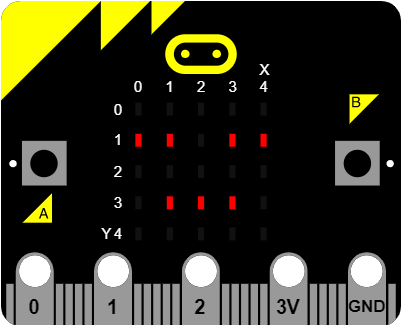
\includegraphics{asleep.png}
\end{center}
\end{figure}

Όταν κάποιος παίκτης πατήσει το δικό του κουμπί εμφανίζεται για 5 δευτερόλεπτα το Α ή το Β αντίστοιχα.
\begin{figure}[!h]
\begin{center}
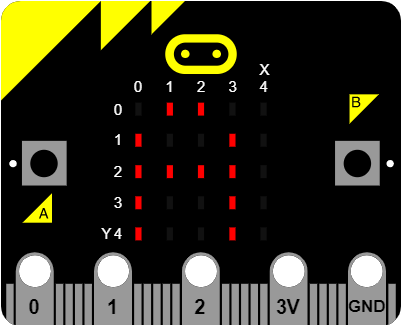
\includegraphics{a.png}\hspace{5em}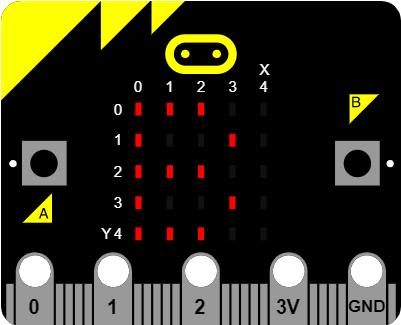
\includegraphics{b.png}
\caption{Image.ASLEEP}
\end{center}
\end{figure}

Το παρακάτω πρόγραμμα υλοποιεί αυτή τη λειτουργία:
\begin{lstlisting}
#buzzer
#show the fastest of two players
from microbit import *

display.scroll('Buzzer', wait = True)

while True:
    display.show(Image.ASLEEP)
    if button_a.is_pressed():
        display.show('A')
        sleep(5000)
    if button_b.is_pressed():
        display.show('B')
        sleep(5000)
\end{lstlisting}

Ο λογική του προγράμματος είναι να δείχνει την εικόνα \lstinline{Image.ASLEEP}, να ελέγχει αν πατήθηκε το Α και στη συνέχεια να ελέγχει αν πατήθηκε το Β. Όταν δεν πατιέται κανένα κουμπί εμφανίζεται η εικόνα \lstinline{Image.ASLEEP}  με την εντολή:
\begin{lstlisting}[firstnumber=8]
display.show(Image.ASLEEP)
\end{lstlisting}
για κάθε ένα από τα κουμπιά το πρόγραμμα ελέγχει αν πατήθηκε και αν πατήθηκε το εμφανίζει με την εντολή \lstinline{display.show}  στη συνέχεια το micro:bit δεν κάνει τίποτα για 5 δευτερόλεπτα που είναι 5000 χιλιοστά του δευτερολέπτου \lstinline{sleep(5000)} ώστε να προλάβουμε να δούμε το Α ή το Β.
\section{Ένα ζάρι}
Πατώντας το κουμπί Α στην οθόνη του micro:bit εμφανίζεται το πάνω μέρος ενός ζαριού από το 1 έως το 6 όπως αυτά φαίνονται στις παρακάτω εικόνες.
\begin{figure}[!h]
\begin{center}
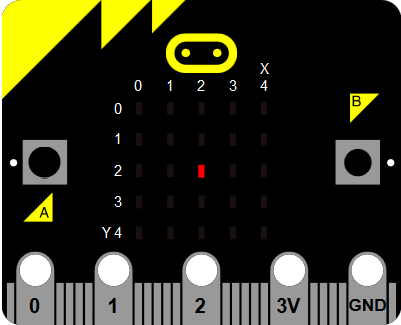
\includegraphics[scale=0.3]{die1.png}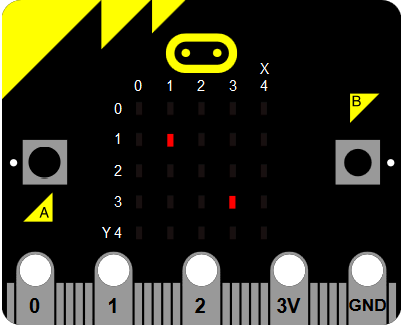
\includegraphics[scale=0.3]{die2.png}\\
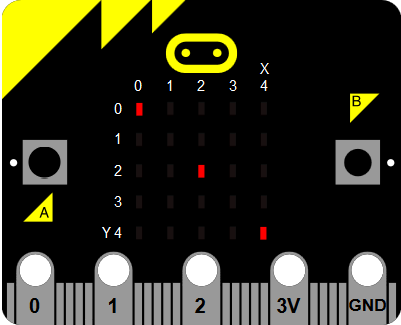
\includegraphics[scale=0.3]{die3.png}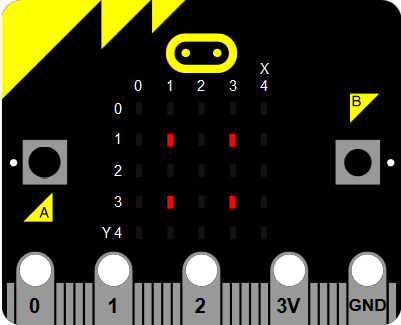
\includegraphics[scale=0.3]{die4.png}\\
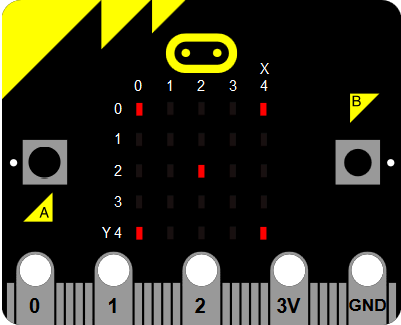
\includegraphics[scale=0.3]{die5.png}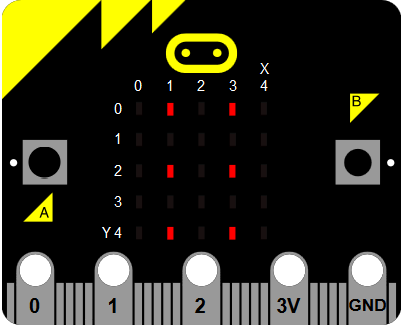
\includegraphics[scale=0.3]{die6.png}
\end{center}
\end{figure}

\begin{lstlisting}
#die
#throws a die
from microbit import *
import random

display.scroll('A Die', wait = True)

def getDiceImage(num):
    num2images = {
        1: '00000:00000:00900:00000:00000',
        2: '00000:09000:00000:00090:00000',
        3: '90000:00000:00900:00000:00009',
        4: '00000:09090:00000:09090:00000',
        5: '90009:00000:00900:00000:90009',
        6: '09090:00000:09090:00000:09090'}
    if num < 1 or num > 6:
        display.show(Image.SAD)
        return(None)
    return(Image(num2images[num]))
 
while True:
    if button_a.was_pressed():
        display.clear()
        sleep(500)
        display.show(getDiceImage(random.randint(1,6)))
\end{lstlisting}

Η συνάρτηση \lstinline{getDiceImage} παίρνει σαν όρισμα έναν αριθμό \lstinline{num} και επιστρέφει την εικόνα του.
Όταν πατιέται το κουμπί Α τότε η οθόνη του micro:bit δεν δείχνει τίποτα για μισό δευτερόλεπτο και μετά δείχνει μια 
από τις έξι εικόνες με τυχαίο τρόπο.


\section{Ζάρια}
Το micro:bit ρίχνει δύο ζάρια και τα εμφανίζει το ένα μετά το άλλο.
\begin{lstlisting}
#dice
#Throws two dice
from microbit import *
import random

display.scroll('Dice', wait = True)

def getDiceImage(num):
    num2images = {
        0: '00000:00000:00000:00000:00000',
        1: '00000:00000:00900:00000:00000',
        2: '00000:09000:00000:00090:00000',
        3: '90000:00000:00900:00000:00009',
        4: '00000:09090:00000:09090:00000',
        5: '90009:00000:00900:00000:90009',
        6: '09090:00000:09090:00000:09090'}
    if num < 0 or num > 6:
        display.show(Image.SAD)
        return(None)
    return(Image(num2images[num]))

dice1 = 0
dice2 = 0
while True:
    if button_a.was_pressed():
        display.clear()
        sleep(500)
        dice1 = random.randrange(1,6)
        dice2 = random.randrange(1,6)
        ar = [getDiceImage(dice1),getDiceImage(dice2)]
        display.show(ar, wait = False, loop = True, clear = True, delay = 600)
\end{lstlisting}

Η εντολή \lstinline{display.show} μπορεί να δείχνει και μια λίστα από εικόνες. Τη λίστα αυτή τη σχηματίζουμε με την εντολή \lstinline{ar = ...} και στη συγκεκριμένη περίπτωση η λίστα περιέχει μόνο δύο εικόνες  (τα δύο ζάρια). Στην εντολή 
\lstinline{display.show} ορίζoυμε να κάνει επανάληψη μεταξύ των δύο εικόνων \lstinline{loop = True}  και να δείχνει την κάθε μία
για 0.6 δευτερόλεπτα \lstinline{delay = 600}.
\end{document}